\documentclass[../main.tex]{subfiles}


\begin{document}
	\section{Úvod do prostředí Robot Mesh studio}

	Našeho robota budeme programovat v prostředí Robot Mesh studio, které je zdarma dostupné na webové stránce \href{https://www.robotmesh.com/studio}{https://www.robotmesh.com/studio}. Robota lze přes toto prostředí programovat v několika jazycích, pro nás budou nejdůležitější \textbf{Blocky} a \textbf{Python}.

	V rámci této kapitoly se naučíme:
	\begin{itemize}
		\item vytvářet nové projekty,
		\item připojovat robota, aby s ním šlo v prostředí komunikovat a
		\item spouštět základní programy v jazyce \textbf{Blocky}.
	\end{itemize}

	\subsection{Vytváření nového projektu}

	Otevřete stránku \href{https://www.robotmesh.com/studio}{https://www.robotmesh.com/studio} v libovolném webovém prohlížeči.

	\begin{figure}[h!]
		\centering
		\frame{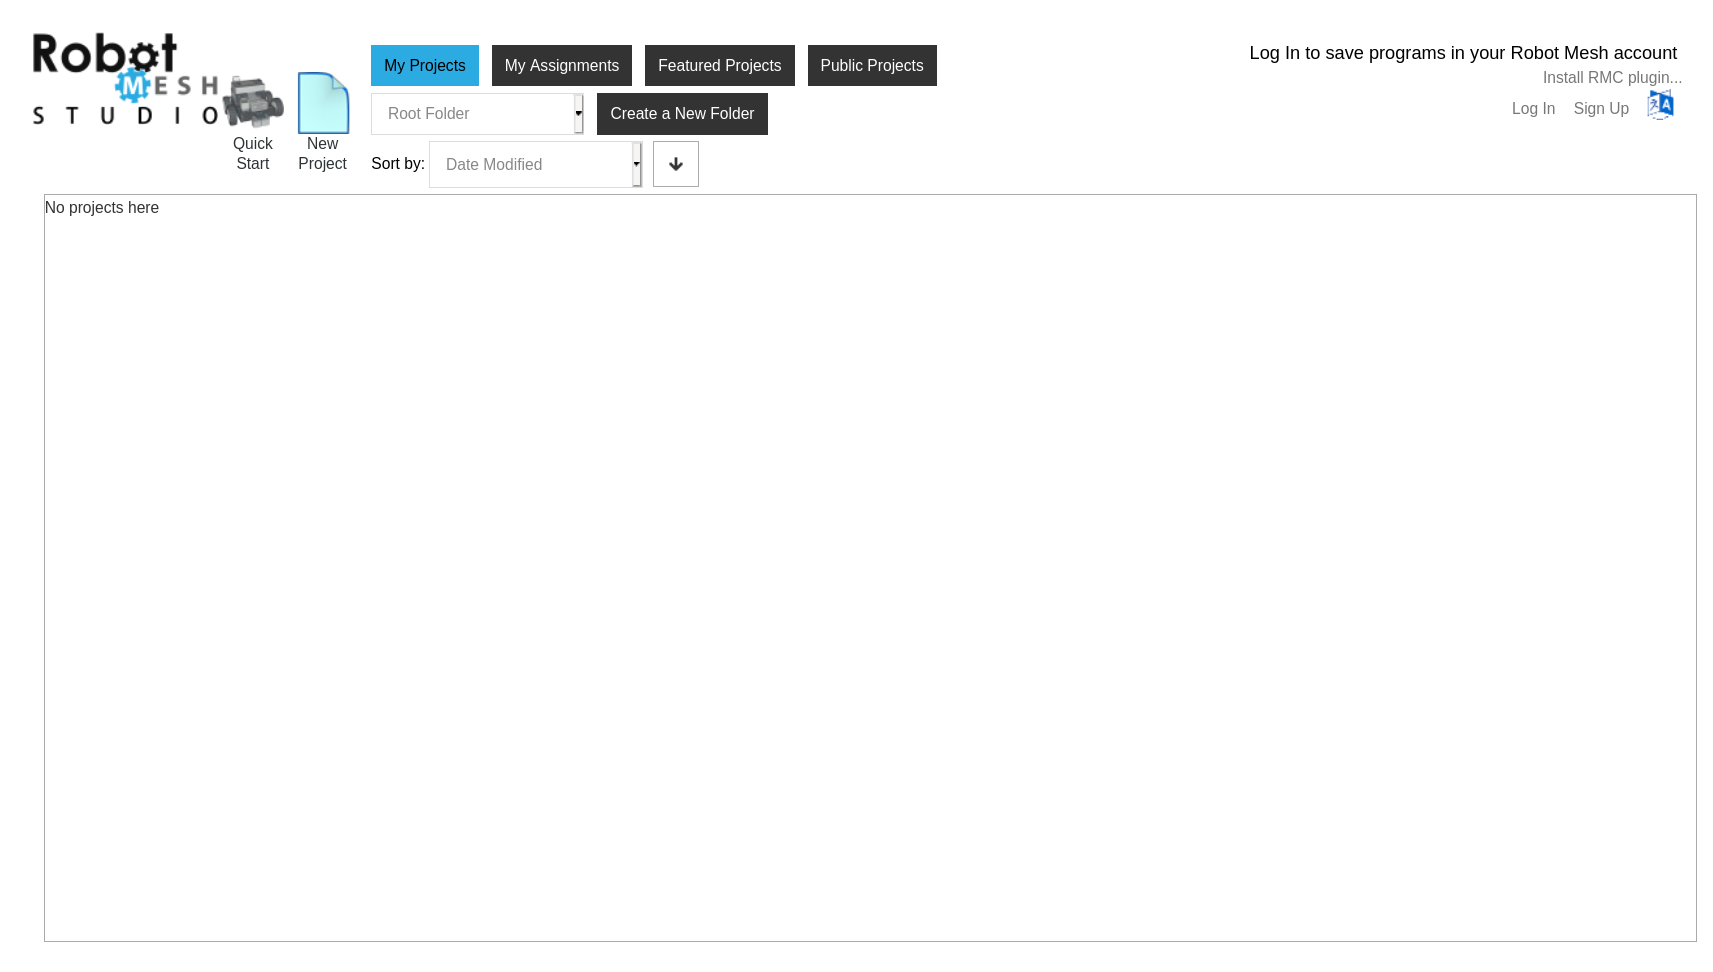
\includegraphics[width=\linewidth]{../Images/01/default-robotmesh-website.png}}
	\end{figure}

	K vytvoření nového projektu stačí kliknout na \textbf{New Project} a poté:

	\begin{figure}[h!]%
		\begin{subfigure}{.3\textwidth}%
			\centering%
			\frame{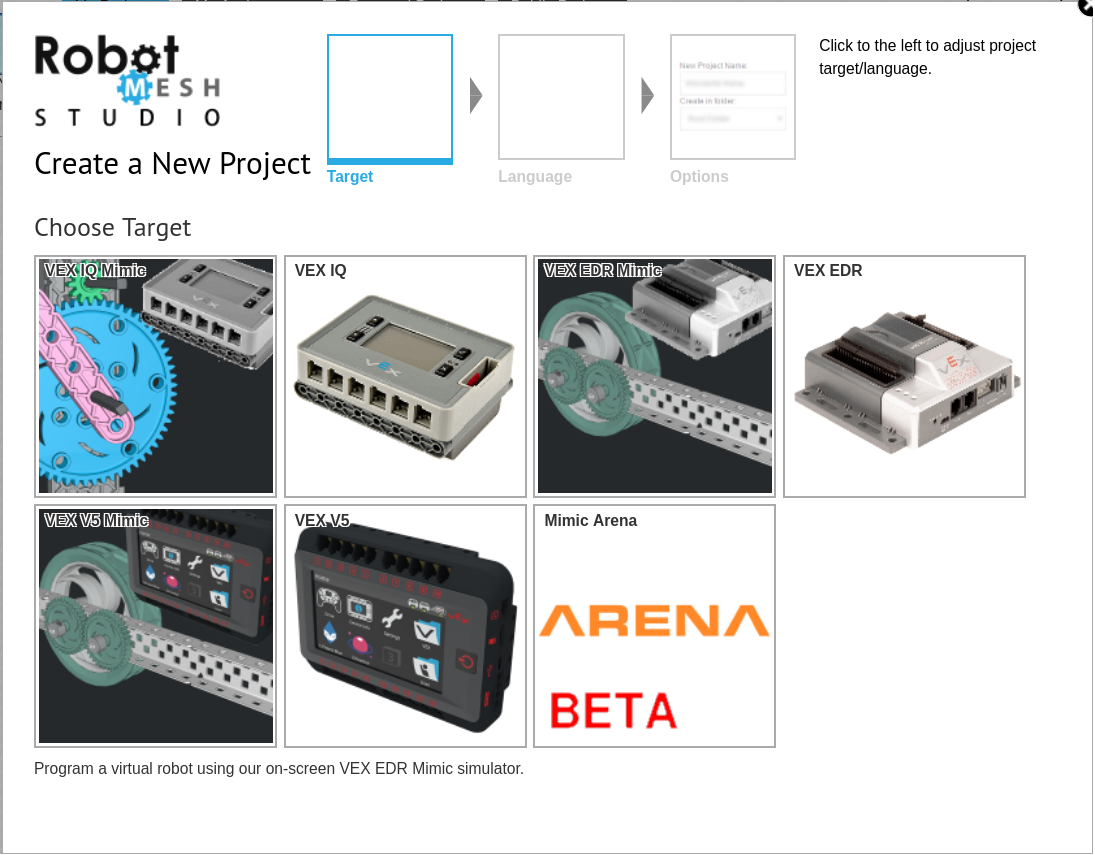
\includegraphics[width=\linewidth]{../Images/01/create-project-1.png}}%
			\caption{kliknout na \textbf{VEX V5}}%
		\end{subfigure} \hspace{.045\textwidth}%
		\begin{subfigure}{.3\textwidth}%
			\centering%
			\frame{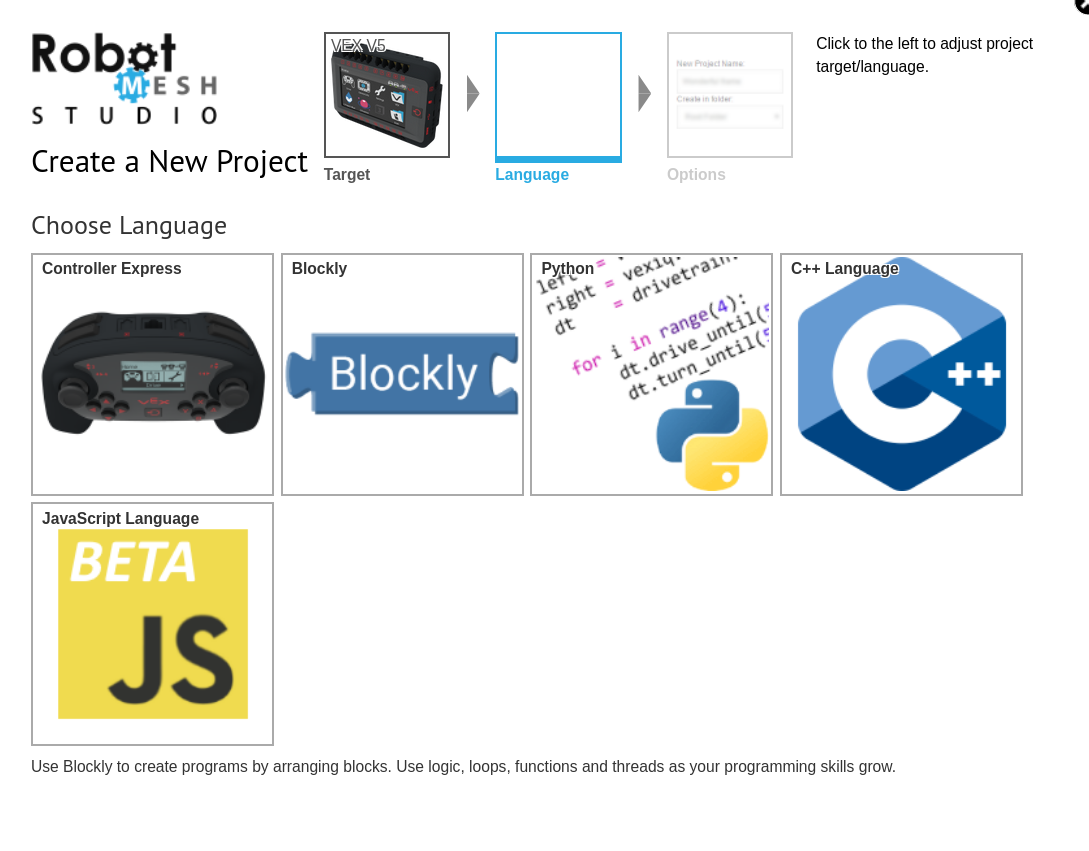
\includegraphics[width=\linewidth]{../Images/01/create-project-2.png}}
			\caption{kliknout na \textbf{Blocky}}%
		\end{subfigure} \hspace{.045\textwidth}%
		\begin{subfigure}{.3\textwidth}%
			\centering%
			\frame{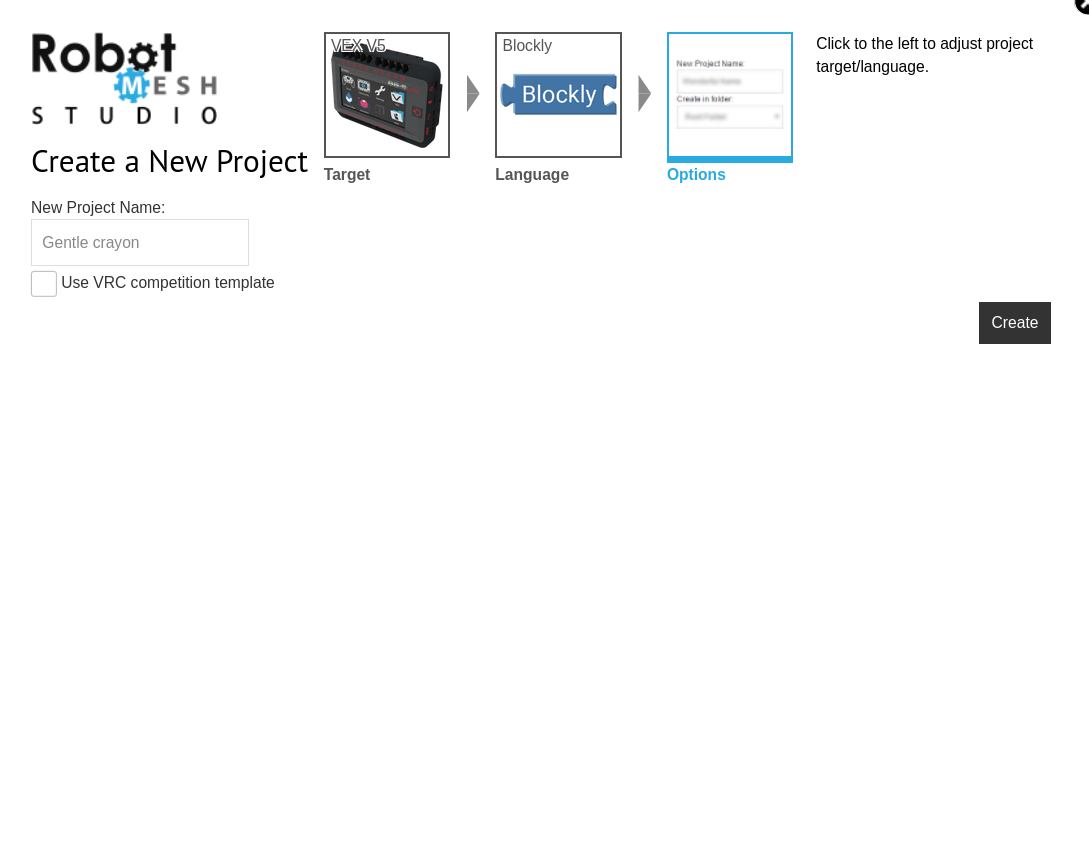
\includegraphics[width=\linewidth]{../Images/01/create-project-3.png}}%
			\caption{kliknout na \textbf{Create}}%
		\end{subfigure}%
	\end{figure}

	\newpage

	Nyní se nacházíme v samotném Robot Mesh studiu. Skládá se z několika částí:

	\begin{itemize}
		\item \textbf{Horní (ovládací) část} -- slouží ke spouštění, pozastavování a zastavování programu.
		\item \textbf{Levá (příkazová) část} -- obsahuje příkazy k ovládání robota, kterými ho budeme ovládat.
		\item \textbf{Pravá (hardwarová) část} -- obsahuje nastavení motorů/senzorů (hardwaru).
		\item \textbf{Prostřední (programová) část} -- obsahuje samotný program.
		\item \textbf{Dolní (statusová) část} -- vypisuje chybové hlášky/oznámení o běhu programu.
	\end{itemize}

	\begin{figure}[h!]
		\centering
		\frame{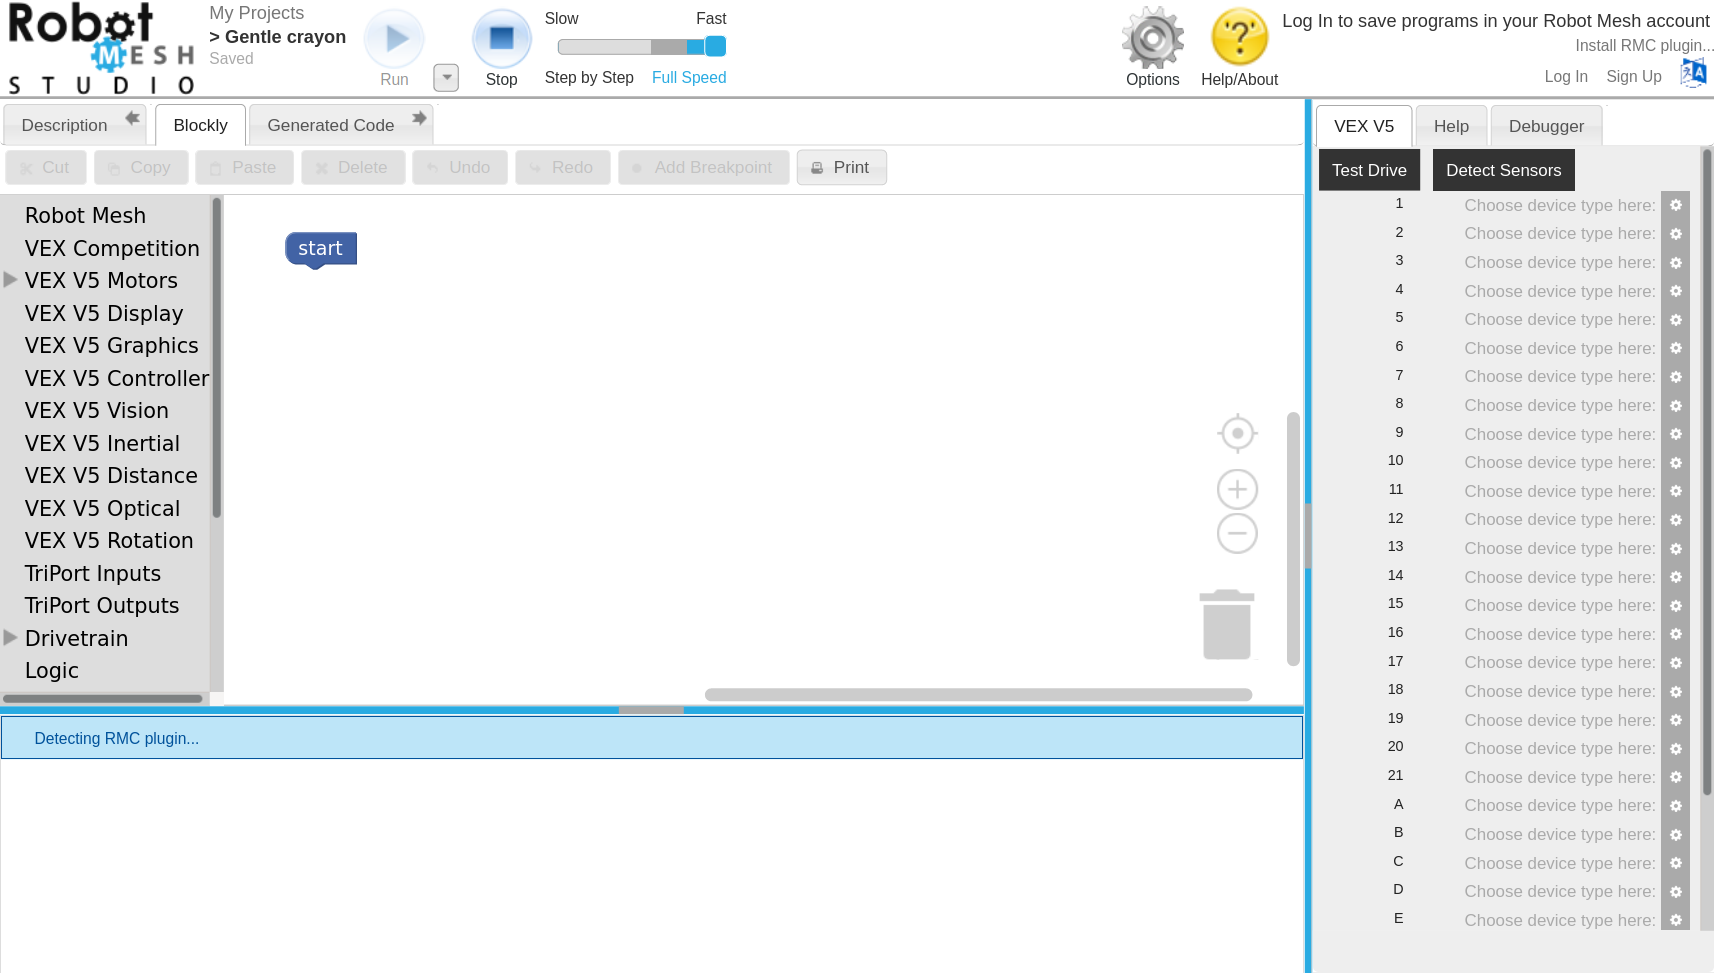
\includegraphics[width=\linewidth]{../Images/01/default-robotmesh-studio.png}}
	\end{figure}

	\subsection{Nastavení robota}

	TODO: připojit robota
	TODO: instalace pluginu
	TODO: funkční prohlížeče

	\subsection{Náš první Blocky program}

	Programovací jazyk Blocky funguje na principu „bloků.“ Program vždy začíná v bloku \tcbox[colback=ceruleanblue,coltext=white]{start} a poté pokračuje do bloku, který je pod tím, který právě dokončil. Jde si to představit například tak, že se jedná o postup k přípravě koláče: pokyny se vykonávají postupně, odshora dolů.

	TODO: nějaký basic program na zapnutí motorů

	\subsection{Programování virtuálního robota}
	Jedna z alternativ k programování reálného robota (toho doma každý k dispozici nemá...) je stránka \href{http://www.robotmesh.com/create/176384}{Hour of Code}, na které je možné programy psát a vykonávat na virtuálním robotovi v simulaci.

	\begin{figure}[h!]%
		\begin{subfigure}{.49\textwidth}%
			\centering%
			\frame{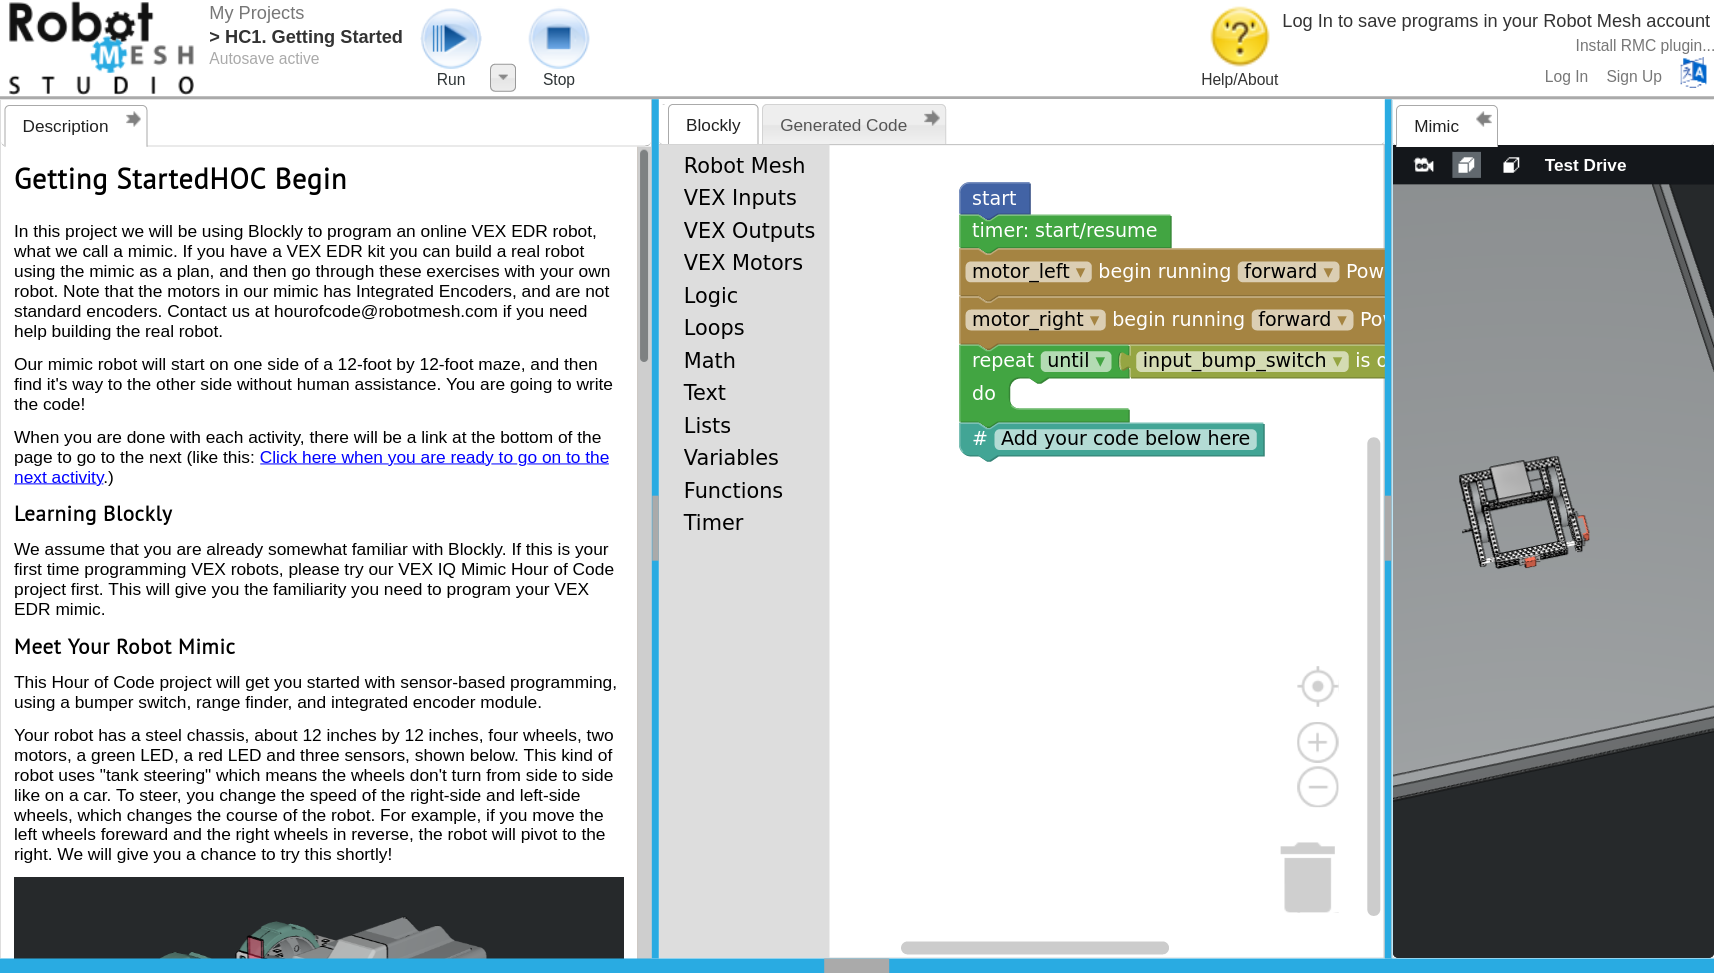
\includegraphics[width=\linewidth]{../Images/01/hour-of-code.png}}%
			\caption{Základní vzhled}%
		\end{subfigure} \hspace{.05\textwidth}%
		\begin{subfigure}{.49\textwidth}%
			\centering%
			\frame{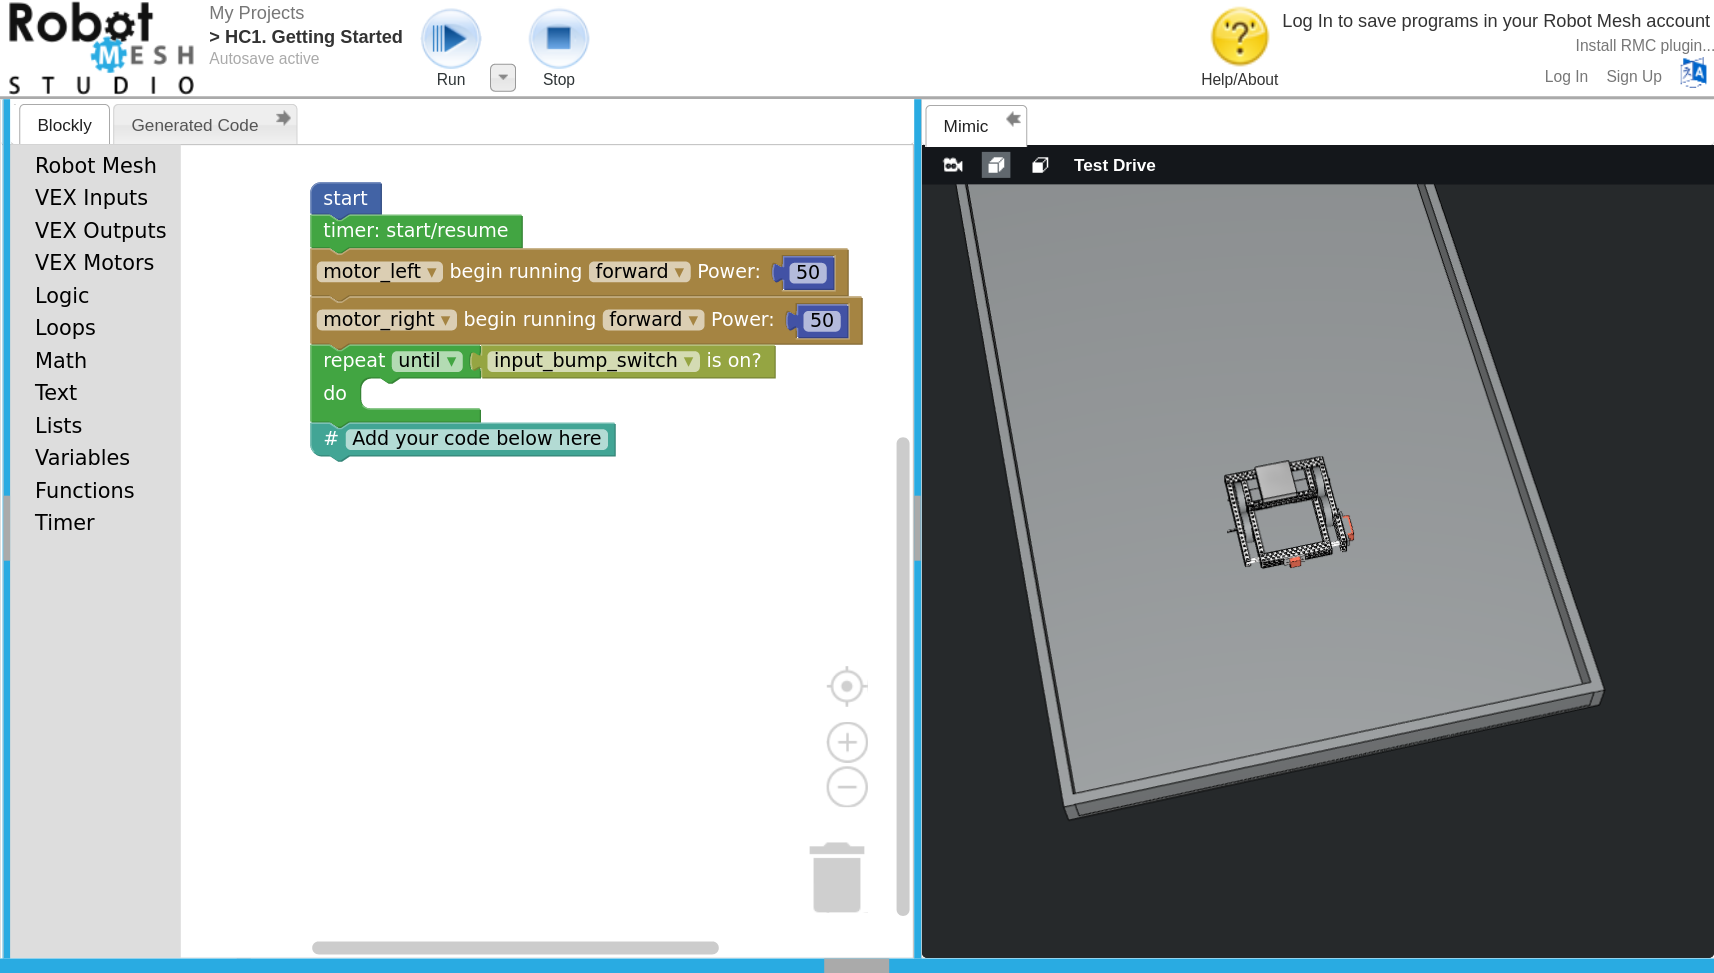
\includegraphics[width=\linewidth]{../Images/01/hour-of-code-uimproved.png}}%
			\caption{Vzhled po posunutí modrých oddělovačů}%
		\end{subfigure}%
		\caption{Stránka \href{http://www.robotmesh.com/create/176384}{Hour of Code}}
	\end{figure}

	Levou stranu s úvodem jde skrýt táhnutím modrého oddělovače, pravou se simulací jde obdobně rozšířit, aby se s robotem a programem lépe pracovalo.

	Je dobré si všimnout, že stránka neobsahuje hardwarovou část, protože není co nastavovat -- virtuální robot má motory a senzory již předdefinované (např. \texttt{motor\_left}, \texttt{motor\_right}).

	Je nutné doplnit, že se jedná o jiný typ robota, než ten, se kterým pracujeme. To ale pro cvičení psaní jednodušších programů v jazyce Blocky vůbec nevadí, protože většina základních konceptů probíraná v následujících kapitolách je identická.

\end{document}
